% !TEX TS-program = pdflatex
% !TEX encoding = UTF-8 Unicode

% This is a simple template for a LaTeX document using the "article" class.
% See "book", "report", "letter" for other types of document.

\documentclass[11pt, titlepage]{article} % use larger type; default would be 10pt

\usepackage[utf8]{inputenc} % set input encoding (not needed with XeLaTeX)

%%% Examples of Article customizations
% These packages are optional, depending whether you want the features they provide.
% See the LaTeX Companion or other references for full information.

%%% PAGE DIMENSIONS
\usepackage{geometry} % to change the page dimensions
\geometry{a4paper} % or letterpaper (US) or a5paper or....
\geometry{margin=2cm, headsep=5mm, includefoot, includehead}

\usepackage{graphicx} % support the \includegraphics command and options

% \usepackage[parfill]{parskip} % Activate to begin paragraphs with an empty line rather than an indent

%%% PACKAGES
\usepackage{booktabs} % for much better looking tables
\usepackage{array} % for better arrays (eg matrices) in maths
\usepackage{paralist} % very flexible & customisable lists (eg. enumerate/itemize, etc.)
\usepackage{verbatim} % adds environment for commenting out blocks of text & for better verbatim
\usepackage{subfig} % make it possible to include more than one captioned figure/table in a single float
% These packages are all incorporated in the memoir class to one degree or another...

%%% HEADERS & FOOTERS
\usepackage{fancyhdr} % This should be set AFTER setting up the page geometry
\pagestyle{fancy} % options: empty , plain , fancy
\fancyhead{}
%%% SECTION TITLE APPEARANCE
\usepackage{sectsty}
\allsectionsfont{\sffamily\mdseries\upshape} % (See the fntguide.pdf for font help)
% (This matches ConTeXt defaults)

%%% ToC (table of contents) APPEARANCE
\usepackage[nottoc,notlof,notlot]{tocbibind} % Put the bibliography in the ToC
\usepackage[titles,subfigure]{tocloft} % Alter the style of the Table of Contents
\renewcommand{\cftsecfont}{\rmfamily\mdseries\upshape}
\renewcommand{\cftsecpagefont}{\rmfamily\mdseries\upshape} % No bold!

\usepackage{lastpage}
\usepackage{rotating}
%---------- Enable IEEEtran.bst configurations ------
\usepackage{IEEEtrantools}
%----------------------------------------------------

%%% END Article customizations

%%% The "real" document content comes below...

%%% Header %%%%%%%%%%%%%%%%%%%%%%%%%%%%%
\setlength{\headheight}{52.4842pt}
\lhead{EH2760 Management of Projects \\
       Assignment 1 \\
       ESS-CAR/ESS-NW \\
       Leon Fernandez, leonfe@kth.se}
\rhead{Status Report 1 \\
       \today \\
       Version 1 \\
       \thepage(\pageref{LastPage})}
\renewcommand{\headrulewidth}{0.4pt}
%%%%%%%%%%%%%%%%%%%%%%%%%%%%%%%%%%%%%%%%

%%% Footer %%%%%%%%%%%%%%%%%%%%%%%%%%%%%
%\cfoot{blablablabla}
%\renewcommand{\footrulewidth}{0.4pt}
%%%%%%%%%%%%%%%%%%%%%%%%%%%%%%%%%%%%%%%%

%\title{ESS-CAR/ESS-NW Project Plan}
%\author{Jonas Ekman \\
%        Leon Fernandez \\
%        Yini Gao \\
%        Fredrik Hyyrynen \\
%        Jacob Kimblad \\
%        Yifan Ruan
%        }
%\date{} % Activate to display a given date or no date (if empty),
         % otherwise the current date is printed 

\begin{document}
%\maketitle
\bstctlcite{BSTcontrol} % IEEEtran.bst controls enabled


%----------------------------------------------------------------------------------------
%	TITLE PAGE
%----------------------------------------------------------------------------------------
\iffalse
\begin{titlepage} % Suppresses displaying the page number on the title page and the subsequent page counts as page 1
	\newcommand{\HRule}{\rule{\linewidth}{0.5mm}} % Defines a new command for horizontal lines, change thickness here
	
	\center % Centre everything on the page
	
	%------------------------------------------------
	%	Headings
	%------------------------------------------------
	
	\textsc{\LARGE EH2760 Management of Projects}\\[1.5cm] % Main heading such as the name of your university/college
	
	\textsc{\Large ESS-CAR/ESS-NW}\\[0.5cm] % Major heading such as course name
	
	\textsc{\large Stockholm, Sweden}\\[0.5cm] % Minor heading such as course title
	
	%------------------------------------------------
	%	Title
	%------------------------------------------------
	
	\HRule\\[0.4cm]
	
	{\huge\bfseries Status Report 1}\\[0.4cm] % Title of your document
	
	\HRule\\[1.5cm]
	
	%------------------------------------------------
	%	Author(s)
	%------------------------------------------------
	
	\begin{minipage}{0.4\textwidth}
		\begin{flushleft}
			\large
                        \textsc{Jonas Ekman}
			\\
			\textsc{Yini Gao}
                        \\
                        \textsc{Jacob Kimblad}
		\end{flushleft}
	\end{minipage}
	~
	\begin{minipage}{0.4\textwidth}
		\begin{flushright}
			\large
                        \textsc{Leon Fernandez}
			\\
			\textsc{Fredrik Hyyrynen}
                        \\
                        \textsc{Yifan Ruan}
		\end{flushright}
	\end{minipage}
	
	% If you don't want a supervisor, uncomment the two lines below
        % and comment the code above
	%{\large\textit{Author}}\\
	%John \textsc{Smith} % Your name
	
	%------------------------------------------------
	%	Date
	%------------------------------------------------
	
	\vfill\vfill\vfill % Position the date 3/4 down the remaining page
	
	{\large\today} % Date, change the \today to a set date if you want
                       % to be precise
	
	%------------------------------------------------
	%	Logo
	%------------------------------------------------
	
	%\vfill\vfill
	%
\includegraphics[width=0.2\textwidth]{placeholder.jpg}\\[1cm]
        % Include a department/university logo
        % - this will require the graphicx package
	 
	%-------------------------------------------------------------------
	
	\vfill % Push the date up 1/4 of the remaining page
	
\end{titlepage}
\fi
%-------------------------------------------------------------------------


\section*{General Description of Status}
Since the last status report (9th Nov) the prototyping phase has ended. The project is now moving
in to the optimization phase, where all the subsystems will be connected and tweaked for performance.
The general status looks good at the time of writing and no changes to the timeplan has been made since
the last status report.

\section*{Resource Status}
The resource status looks good at the time of writing.

\section*{Problems / Action Plan}
Personal equipment will be in use during the testing (a smartphone). If the stakeholders
wish to demo the car without any project members present, they need to make sure that they
have a smartphone with some software from the project installed on it. The project members
can provide help with this if requested.

\section*{Risks / Action Plan}
The only change to the risk management since last week is that documentation of the project has begun.
README-files, pin diagrams and schematics for the Arduino-based subsystems are mostly completed.
The network architecture of the system has been documented. Code and physical design has yet to be
documented.

\section*{Project Changes From the Project Plan}
No changes to the project plan have been introduced. No new documents have been introduced to the project.

\appendix
\section{EVM}
\begin{figure}[h]
     \centering
     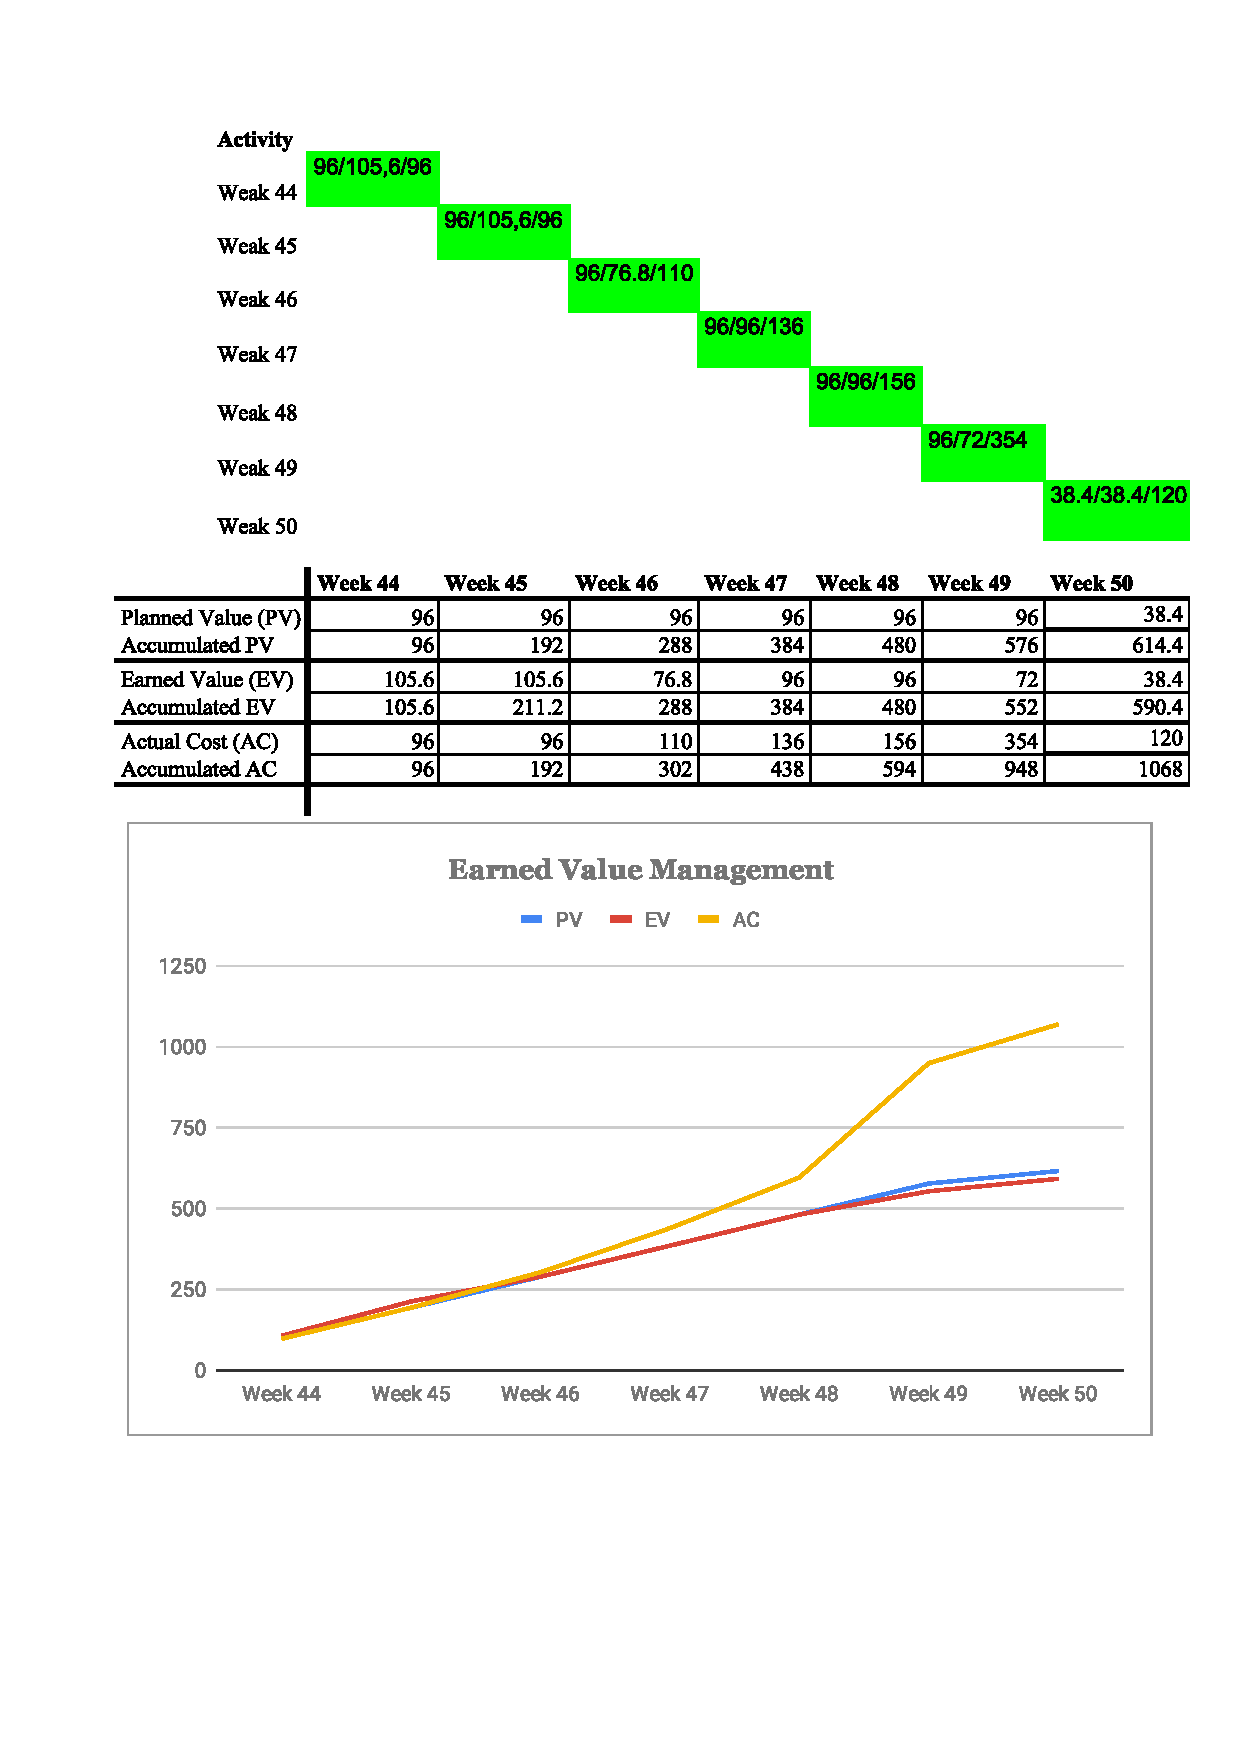
\includegraphics[scale=0.8]{evm.pdf}
     \caption{Earned Value Management analysis.}
     \label{fig:evm}
\end{figure}

\section{Time Plan}
\begin{sidewaysfigure}
     \centering
     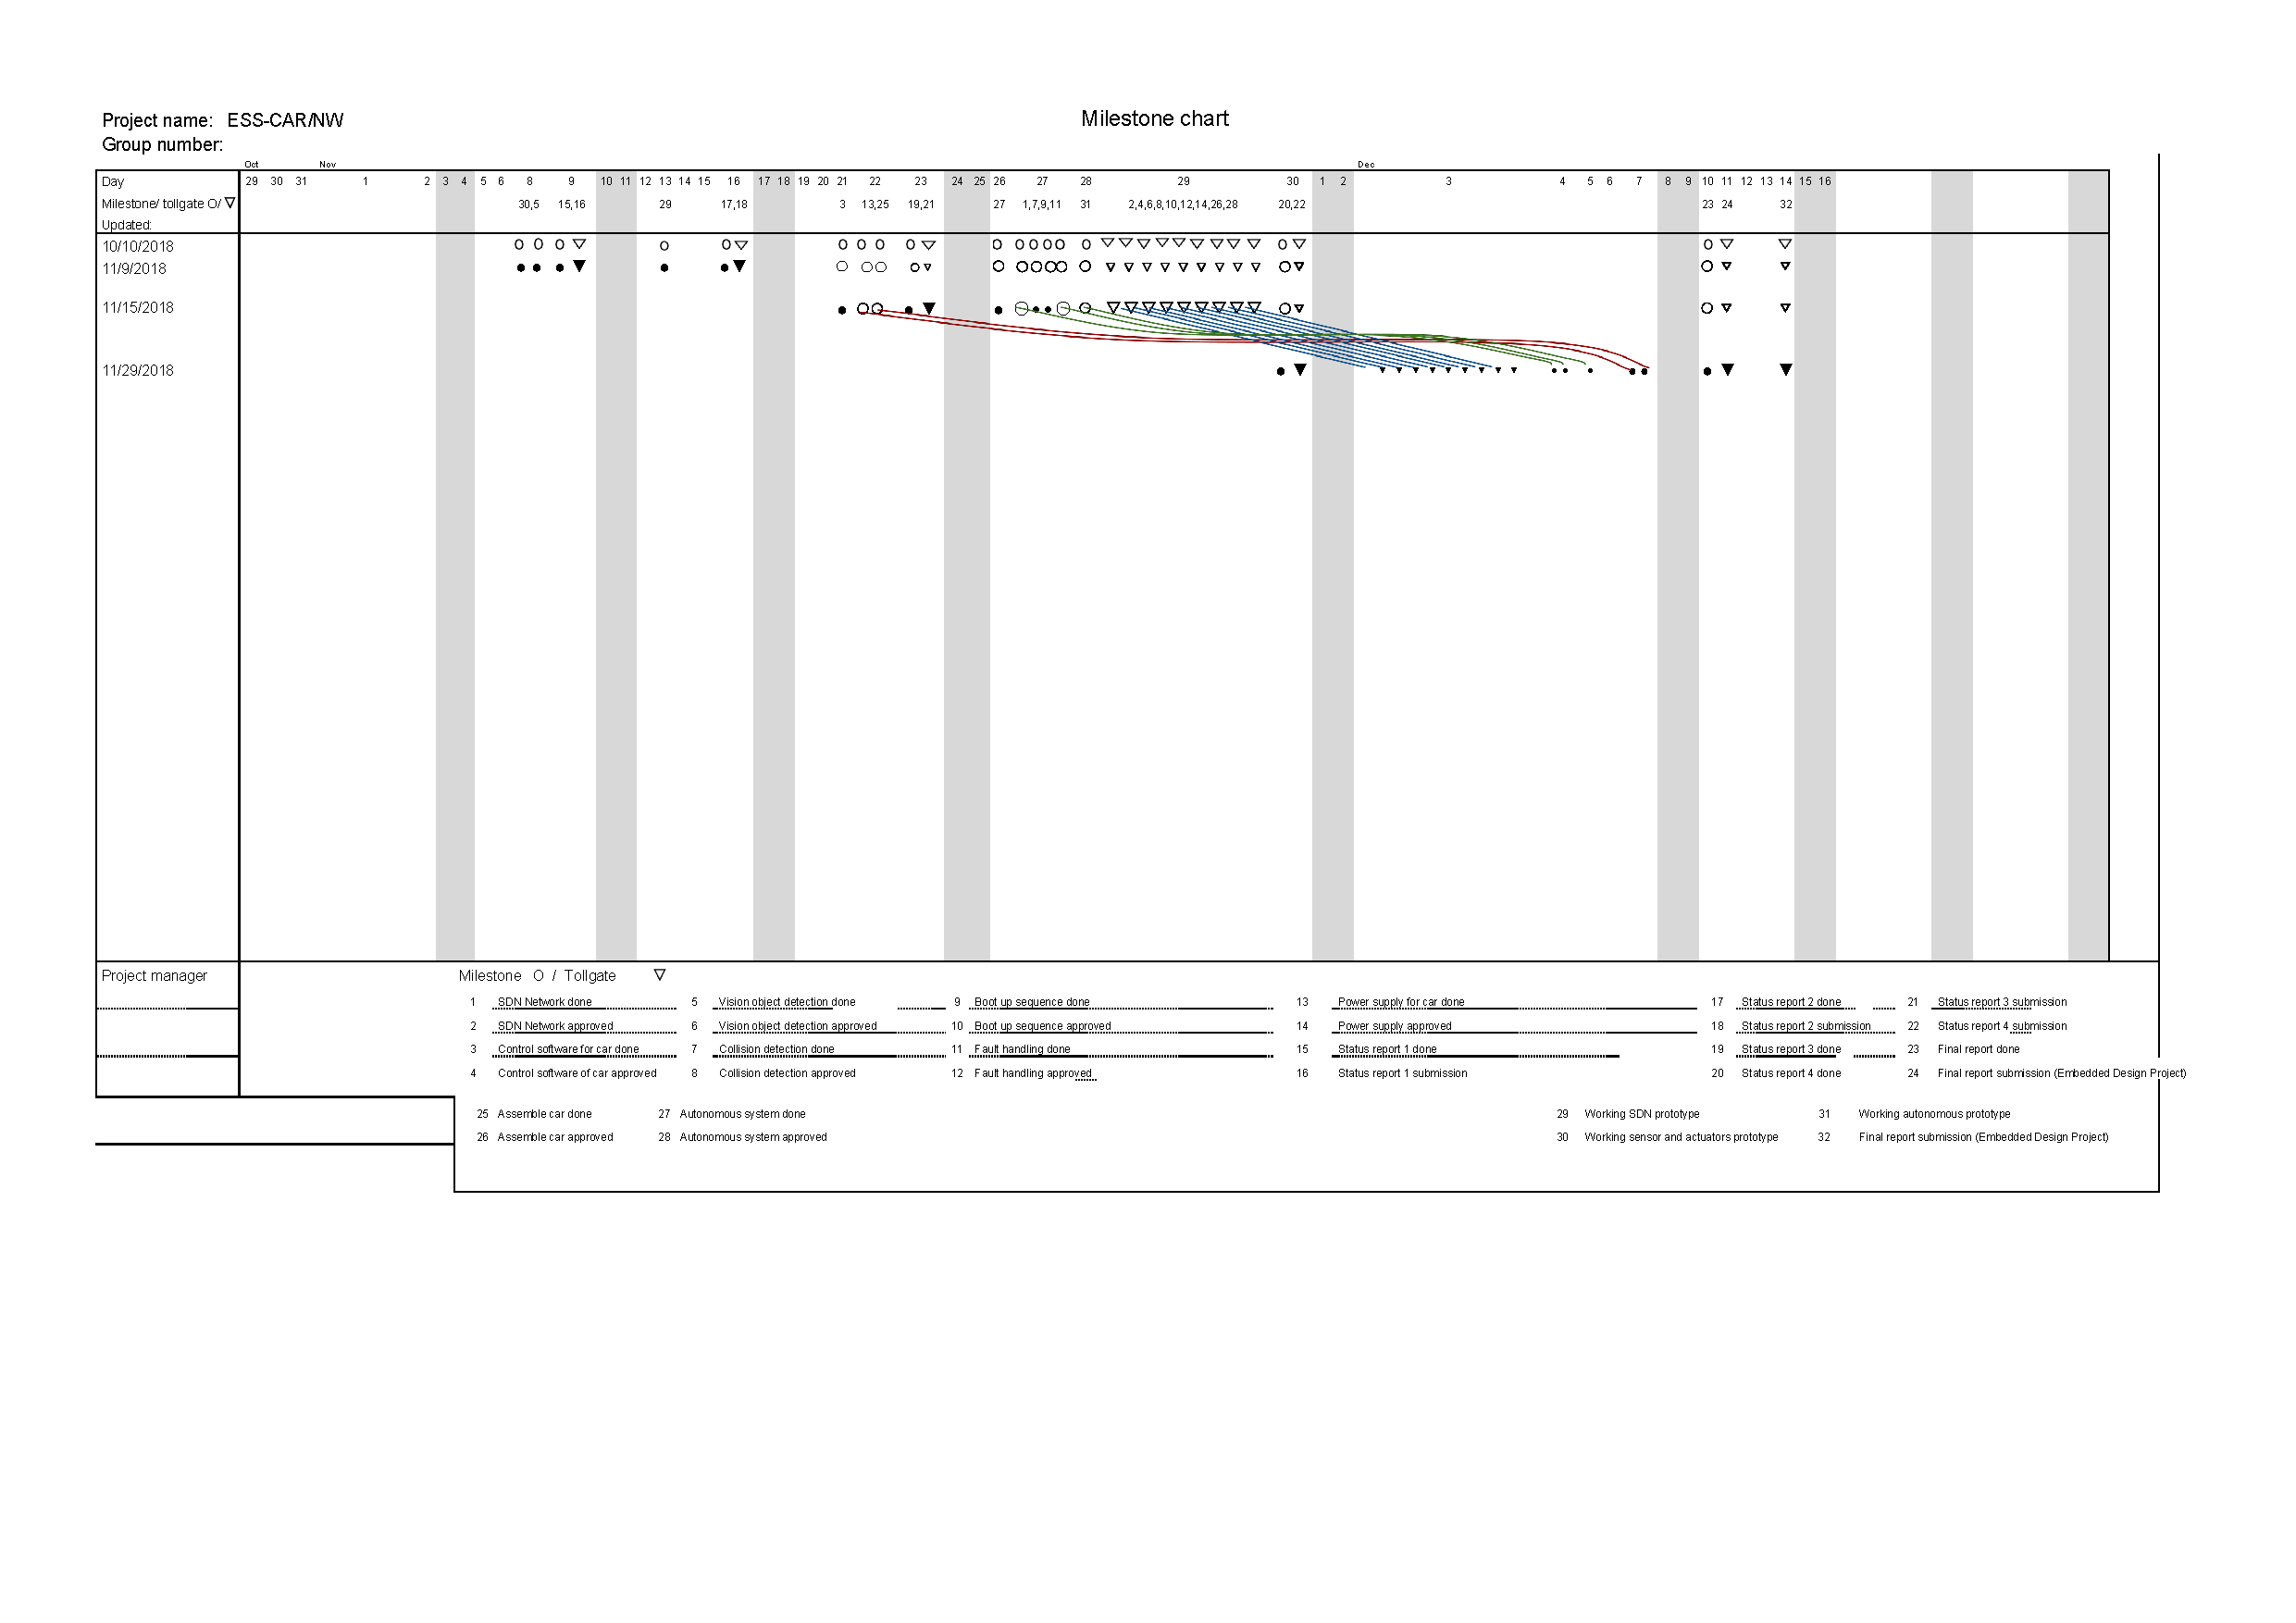
\includegraphics[scale=0.6]{timeplan.pdf}
     \caption{Timeplan for the project.}
     \label{fig:resource}
\end{sidewaysfigure}

\section{Resource Plan}
\begin{sidewaysfigure}
     \centering
     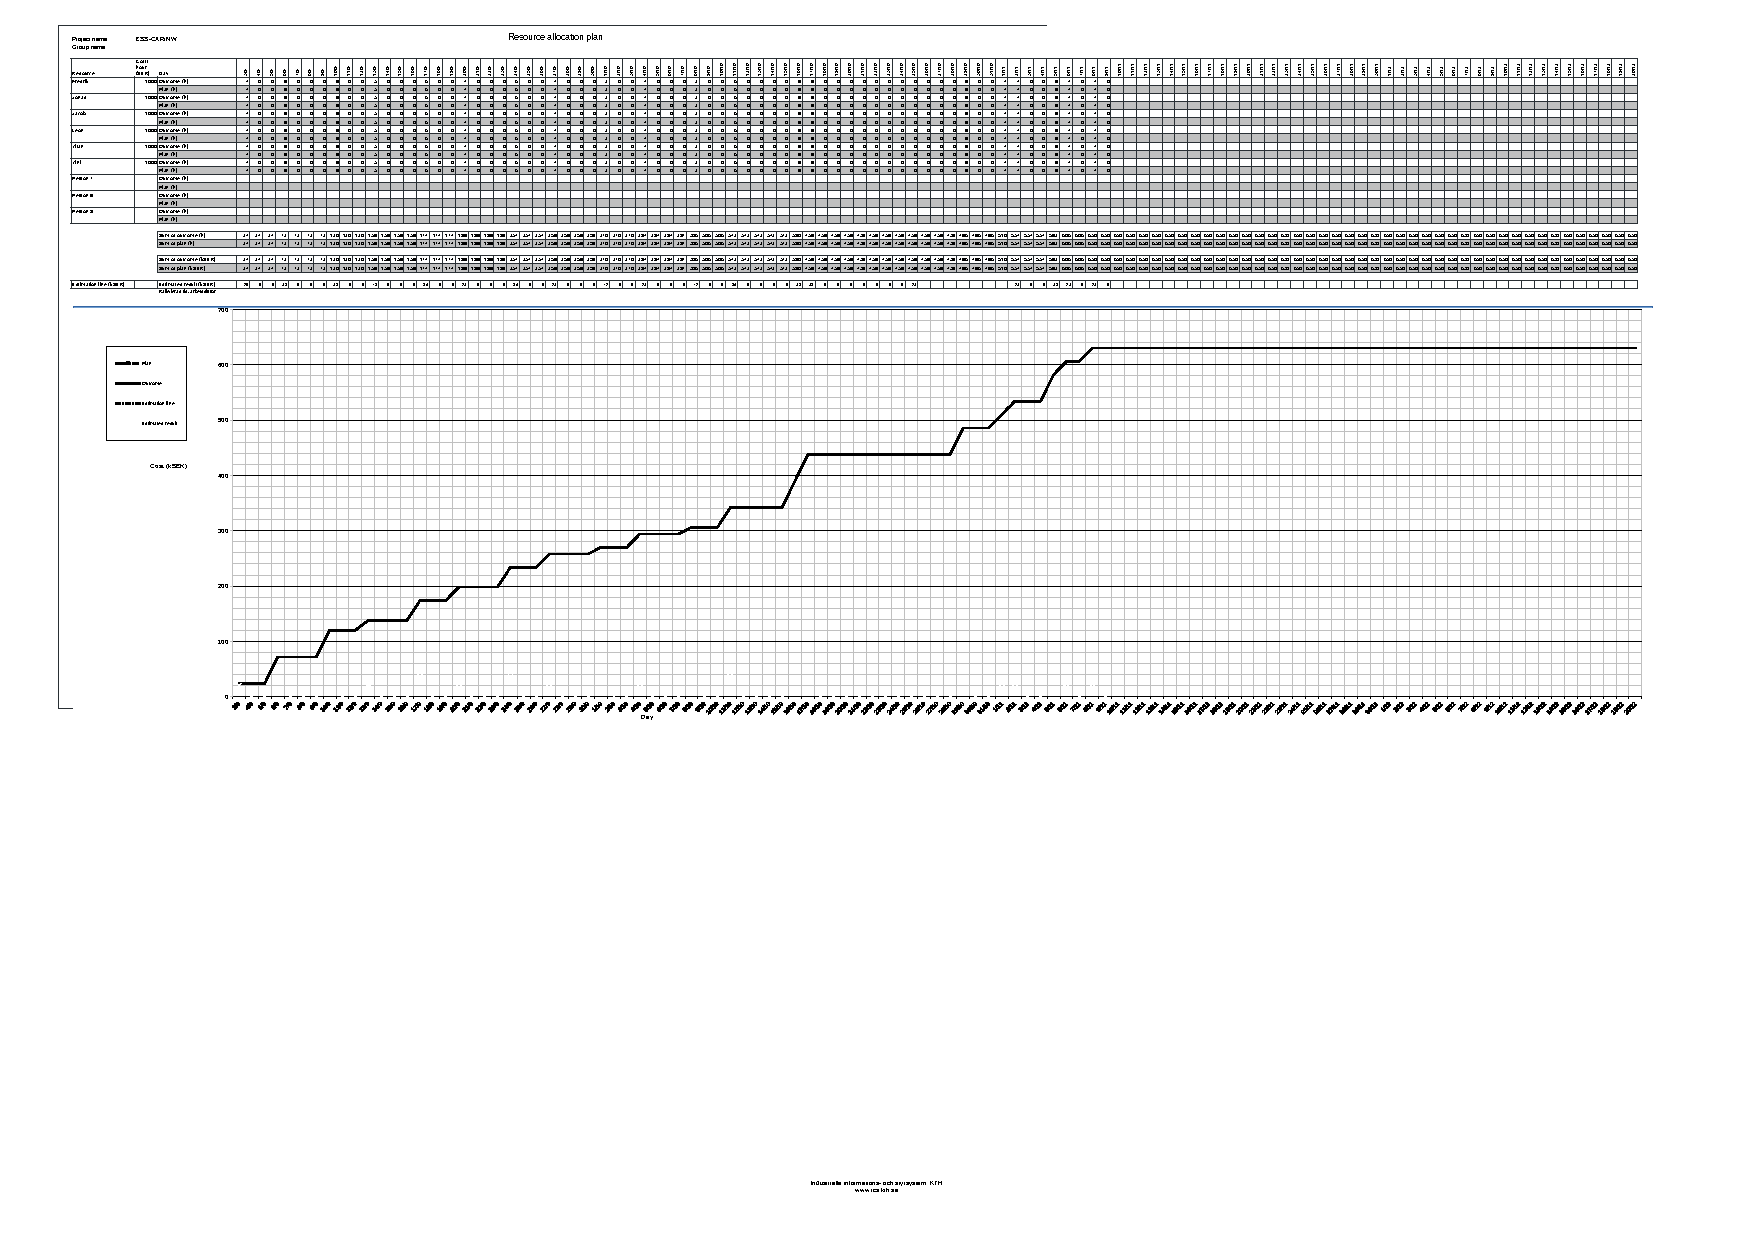
\includegraphics[scale=0.8]{resource_plan.pdf}
     \caption{Resource plan for the project.}
     \label{fig:resource}
 \end{sidewaysfigure}
\end{document}
